\documentclass[slidestop,usenames,dvipsnames]{beamer}
\usepackage[utf8]{inputenc}
\usepackage[T1]{fontenc}
\usepackage{graphicx}
\usepackage[yyyymmdd]{datetime}
\renewcommand{\dateseparator}{-}

\title{Network Cascades}
\subtitle{The Grim Truth Revealed}
\author{Marco Brack \and Carsten Hartenfels}

\beamertemplatenavigationsymbolsempty
\usetheme{Boadilla}
\usecolortheme{whale}
\setbeamertemplate{itemize items}[default]
\setbeamertemplate{enumerate items}[default]
\defbeamertemplate*{footline}{my infolines theme} {
    \leavevmode
    \hbox{
    \begin{beamercolorbox}[wd=.333333\paperwidth,ht=2.25ex,dp=1ex,center]{author in head/foot}
        \usebeamerfont{author in head/foot}Marco Brack, Carsten Hartenfels
    \end{beamercolorbox}
    \begin{beamercolorbox}[wd=.333333\paperwidth,ht=2.25ex,dp=1ex,center]{title in head/foot}
        \usebeamerfont{title in head/foot}The Grim Truth Revealed
    \end{beamercolorbox}
    \begin{beamercolorbox}[wd=.309\paperwidth,ht=2.25ex,dp=1ex,center]{date in head/foot}
        \usebeamerfont{date in head/foot}\insertshortdate{}\hspace*{2em}
        \insertframenumber{} / \inserttotalframenumber\hspace*{2ex}
    \end{beamercolorbox}}
    \vskip0pt
}

\newcommand{\fitem}{\pause\vfill\item}
\newcommand{\gitem}{\vfill\item}

\begin{document}

\begin{frame}
    \titlepage
\end{frame}


%%%%%%%%%%%%%%%%%%%%%%%%%%%%%%%%%%%%%%%%%%%%%%%%


\begin{frame}
    \frametitle{Content}
    \begin{itemize}
        \gitem Sinister Motives
        \gitem Model of Doom
        \gitem The Cascade Into Madness
        \gitem Termination
    \end{itemize}
    \vfill
\end{frame}


\begin{frame}
    \frametitle{Sinister Motives}
    \begin{itemize}
        \fitem How Did Twilight Become Popular?
        \fitem How Did the Turkish Military Start a Coup?
        \fitem How Did WhatsApp Get Users?
        \fitem How Do You Come Up With More Questions Like These??? TODO pls
    \end{itemize}
    \vfill
\end{frame}

\begin{frame}
    \frametitle{Definitely the Evil Mastermind Behind All This}
    \vfill
    \begin{center}
        \pause {\Huge \underline{Network Cascades}}\\
        \vspace{20pt}
        \pause {\footnotesize (Maybe)}\\
        \vspace{20pt}
        \pause {\footnotesize (It's a Nice Model Anyway)}
    \end{center}
    \vfill
\end{frame}


\begin{frame}
    \frametitle{Model of Doom}
    \begin{itemize}
        \gitem Nodes
    \end{itemize}
    \vfill
    \includegraphics[width=\textwidth]{img/model1}
    \vfill
\end{frame}

\begin{frame}
    \frametitle{Model of Doom}
    \begin{itemize}
        \gitem Observe $k$ Neighbors
    \end{itemize}
    \vfill
    \includegraphics[width=\textwidth]{img/model2}
    \vfill
\end{frame}

\begin{frame}
    \frametitle{Model of Doom}
    \begin{itemize}
        \gitem State $\in \lbrace 0, 1 \rbrace$
    \end{itemize}
    \vfill
    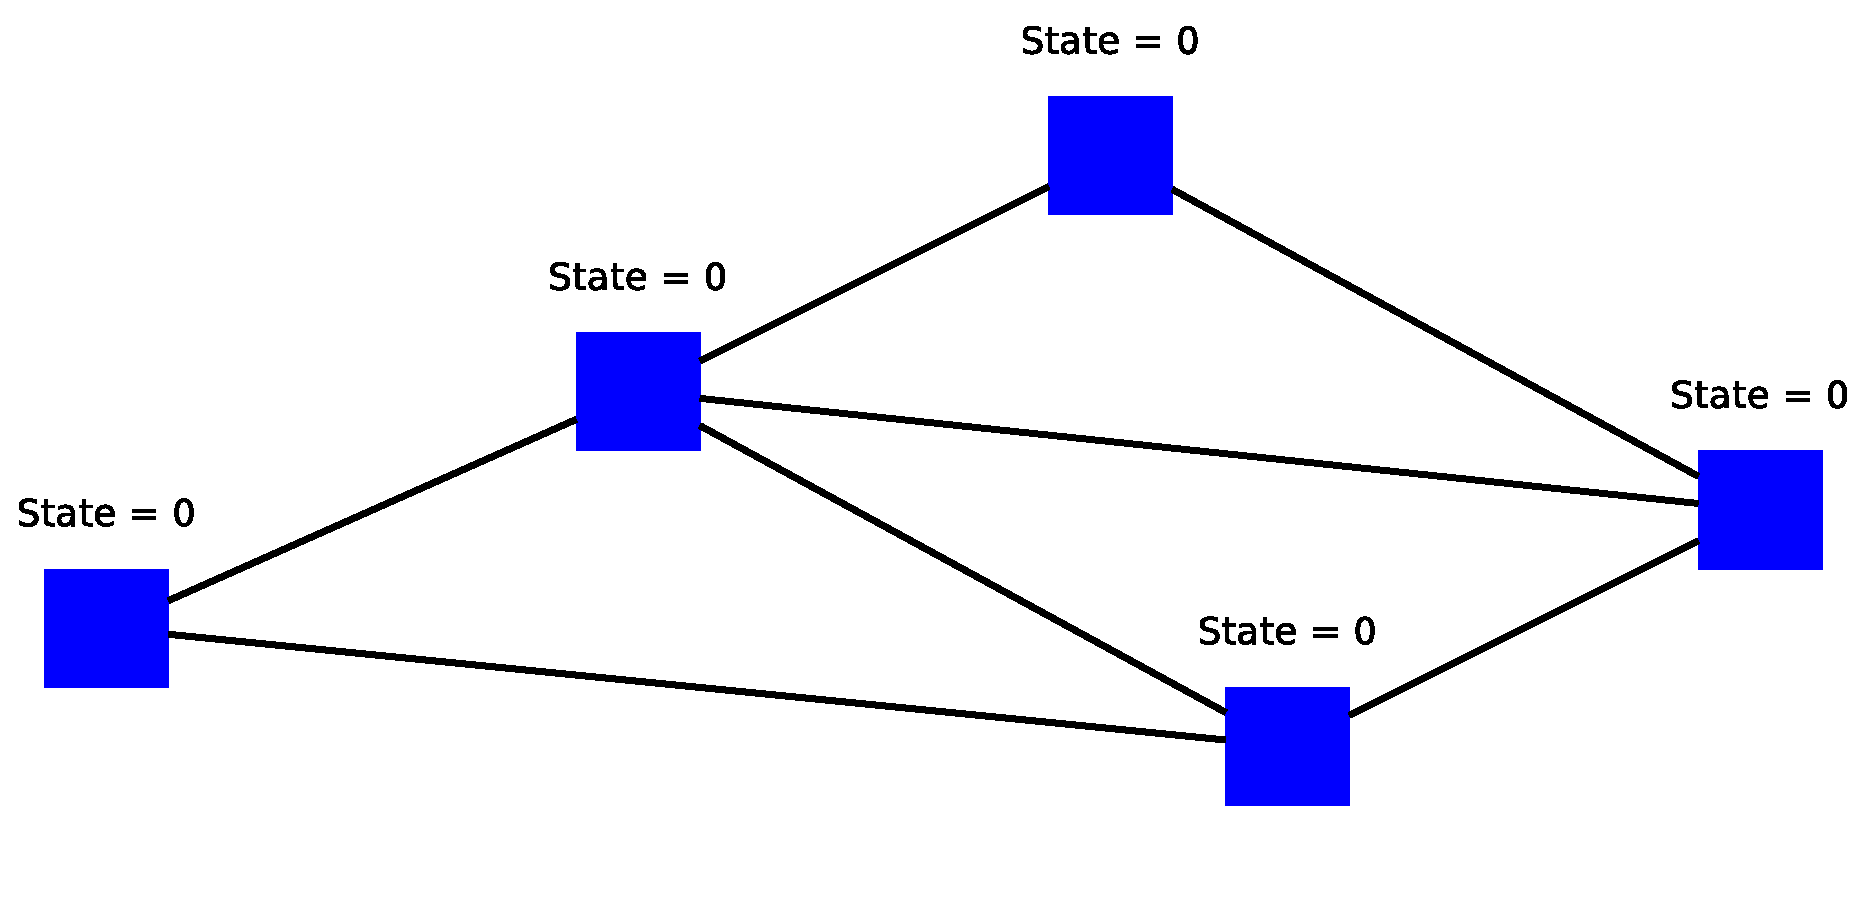
\includegraphics[width=\textwidth]{img/model3}
    \vfill
\end{frame}

\begin{frame}
    \frametitle{Model of Doom}
    \begin{itemize}
        \gitem Threshold $\Phi \in [0, 1]$
    \end{itemize}
    \vfill
    \includegraphics[width=\textwidth]{img/model4}
    \vfill
\end{frame}

\begin{frame}
    \frametitle{Model of Doom}
    \begin{itemize}
        \gitem Random Impulse Happens
    \end{itemize}
    \vfill
    \includegraphics[width=\textwidth]{img/model5}
    \vfill
\end{frame}

\begin{frame}
    \frametitle{Model of Doom}
    \begin{itemize}
        \gitem Nodes Check in Random Intervals
    \end{itemize}
    \vfill
    \includegraphics[width=\textwidth]{img/model6}
    \vfill
\end{frame}

\begin{frame}
    \frametitle{Model of Doom}
    \begin{itemize}
        \gitem Stuff Happens
    \end{itemize}
    \vfill
    \includegraphics[width=\textwidth]{img/model7}
    \vfill
\end{frame}

\begin{frame}
    \frametitle{Model of Doom}
    \begin{itemize}
        \gitem Things Occur
    \end{itemize}
    \vfill
    \includegraphics[width=\textwidth]{img/model8}
    \vfill
\end{frame}

\begin{frame}
    \frametitle{Model of Doom}
    \begin{itemize}
        \gitem Coup Successful
    \end{itemize}
    \vfill
    \includegraphics[width=\textwidth]{img/model9}
    \vfill
\end{frame}


\begin{frame}
    \frametitle{Model of Doom II: Electric Boogaloo}
    \begin{itemize}
        \fitem Nodes Start with State $0$
        \fitem Observe Neighbors in Random Intervals
        \fitem Change State Depending on Threshold
        \fitem Random Impulse of State $1$
    \end{itemize}
    \vfill
\end{frame}


%%%%%%%%%%%%%%%%%%%%%%%%%%%%%%%%%%%%%%%%%%%%%%%%


\begin{frame}
    \vfill
    \begin{center}
        {\Huge Thank You All For Listening}\
    \end{center}
\end{frame}

\end{document}
